\section{2}
\subsection{5}
see figure:\ref{fig:1}
\begin{figure}[h]
    \centering
    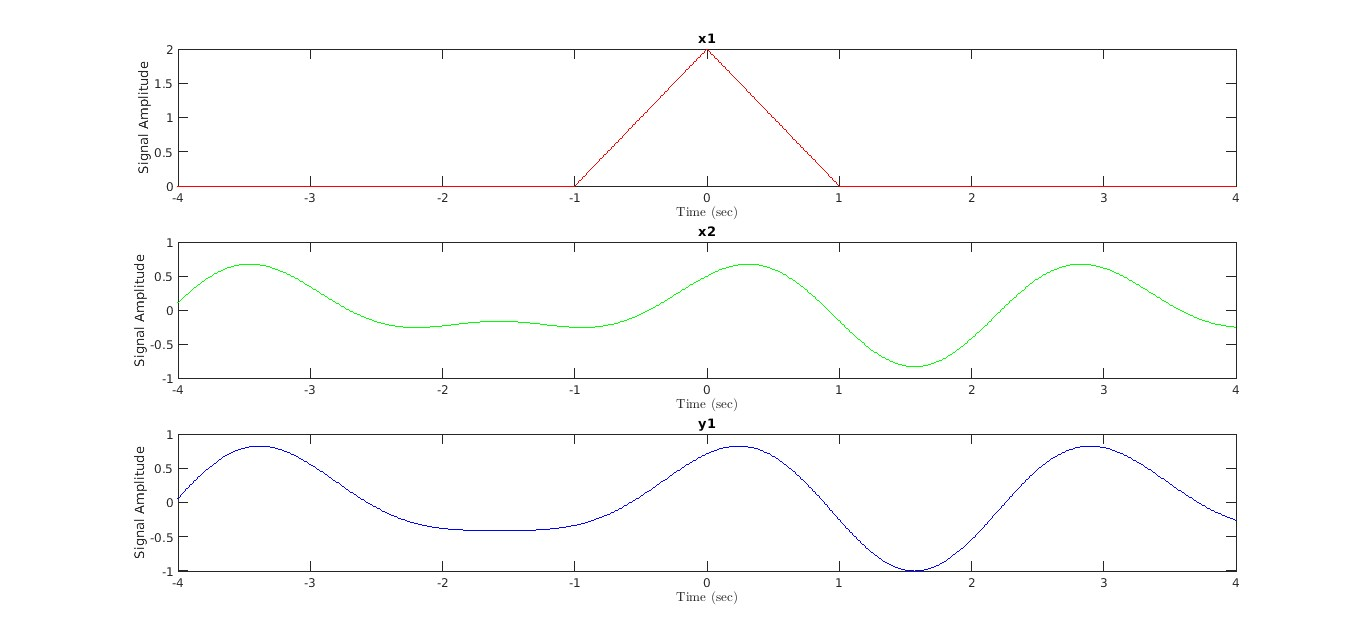
\includegraphics[width=\textwidth]{assets/hw1_2_5.jpg}
    \caption{from top to bottom are the signals $x1$, $x2$, $y1$}
    \label{fig:1}
\end{figure}
\subsection{8}
see figure:\ref{fig:2}
\begin{figure}[h]
    \centering
    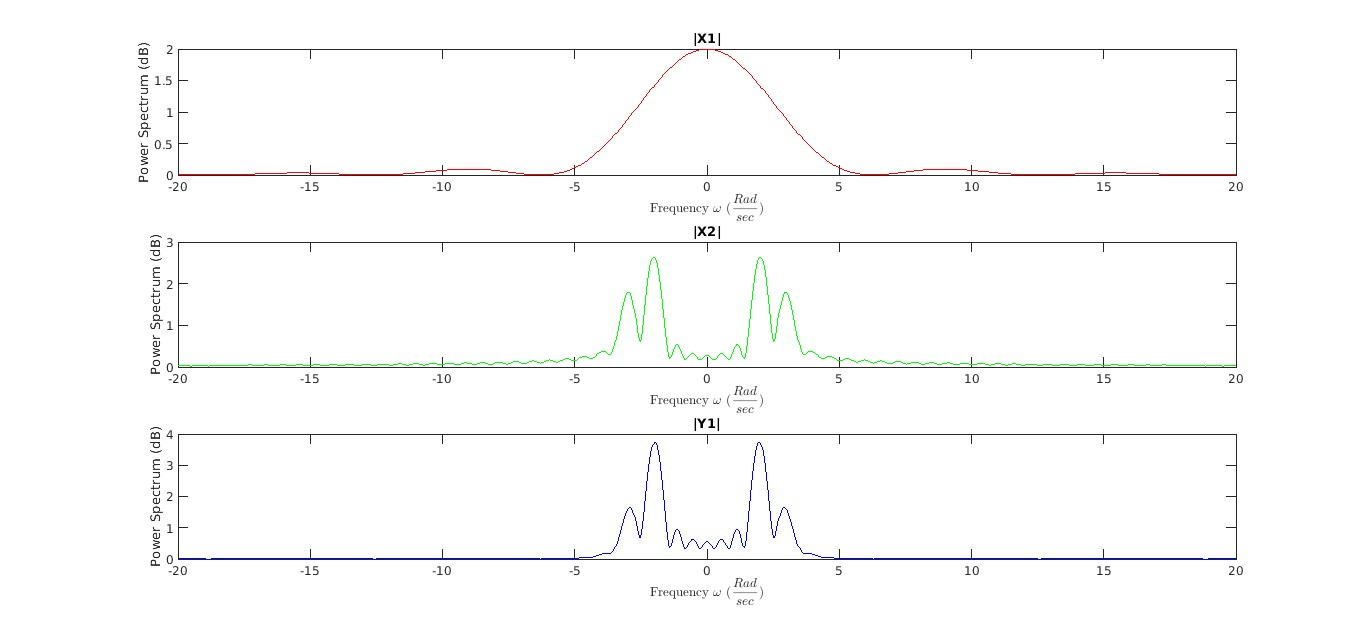
\includegraphics[width=\textwidth]{assets/hw1_2_8.jpg}
    \caption{from top to bottom are graphs of $|X1|$, $|X2|$ and $|Y2|$}
    \label{fig:2}
\end{figure}
\subsection{9}
Yes there are differences between $Y2$ and $y1$ specially at the boundaries of our time interval. This is because the time interval and frequency interval are finite and the fourier transform applied to the signals is an approximation as we can see in figure:\ref{fig:2} with $|X2|$

\section{3}
\subsection{1}
No the system is not linear $\sin(x+y)\neq \sin(x)+\sin(y)$.
But if we use small angle approximation then $\sin(\theta)\approx \theta$ and we get an ODE which in indeed linear.
\subsection{2}
Using small angle approximations the equation is:
\begin{align}
    \theta''(t)=\frac{1}{m l^2}\delta(t)-\frac{g}{l}\theta(t)\\
    \theta''(t)-\frac{g}{l}\theta(t)=\frac{1}{m l^2}\delta(t)
\end{align}
We can use Laplace transform or using Green's function for a harmonic oscillator\footnote{\url{https://phys.libretexts.org/Bookshelves/Mathematical_Physics_and_Pedagogy/Complex_Methods_for_the_Sciences_(Chong)/11\%3A_Green's_Functions/11.01\%3A_The_Driven_Harmonic_Oscillator}}\footnote{we can also solve a simple ODE but changing the initial conditions to $\theta'(0)=\frac{1}{m l^2}$ and $\theta(0)=0$}.
Green's function $G(t,t')$ that satisfies the equation $\left[\frac{\partial^2}{\partial t^2}+2\gamma\frac{\partial}{\partial t}+\omega_0^2\right]G(t,t')=\delta(t-t')$ is of the form:
\begin{equation}
    G(t,t')=j u(t-t')
    \left[
        \frac{e^{-j \om_+(t-t')}}{\om_+-\om_-}+
        \frac{e^{-j \om_-(t-t')}}{\om_--\om_+}
    \right]
    \quad\quad, \om_\pm = -j\gamma \pm \sqrt{\om_0^2-\gamma^2}
\end{equation}
in our case $\om_0=\sqrt{\frac{g}{l}}$, $\gamma=0$,$t'=0$ so $\om_\pm=\pm\om_0$ and $G(t,0)=u(t)\frac{1}{\om_0}\sin(\om_0t)$. Our solution is $\frac{1}{m l^2}G(t,0)$ since the equation is linear, Meaning:
\begin{equation}
    \frac{1}{m l^2}\sqrt{\frac{l}{g}}u(t)\sin(\sqrt{\frac{g}{l}}t).
\end{equation}
\subsection{3}
From the solution above, the frequency of the system is $\frac{1}{2\pi}\sqrt{\frac{g}{l}}\approx 0.557 Hz$
\subsection{4}
Simulation diagram is in figure:\ref{sim:1} and graph of $\theta(t)$ is in figure:\ref{fig:sim1}
\begin{figure}
    \centering
    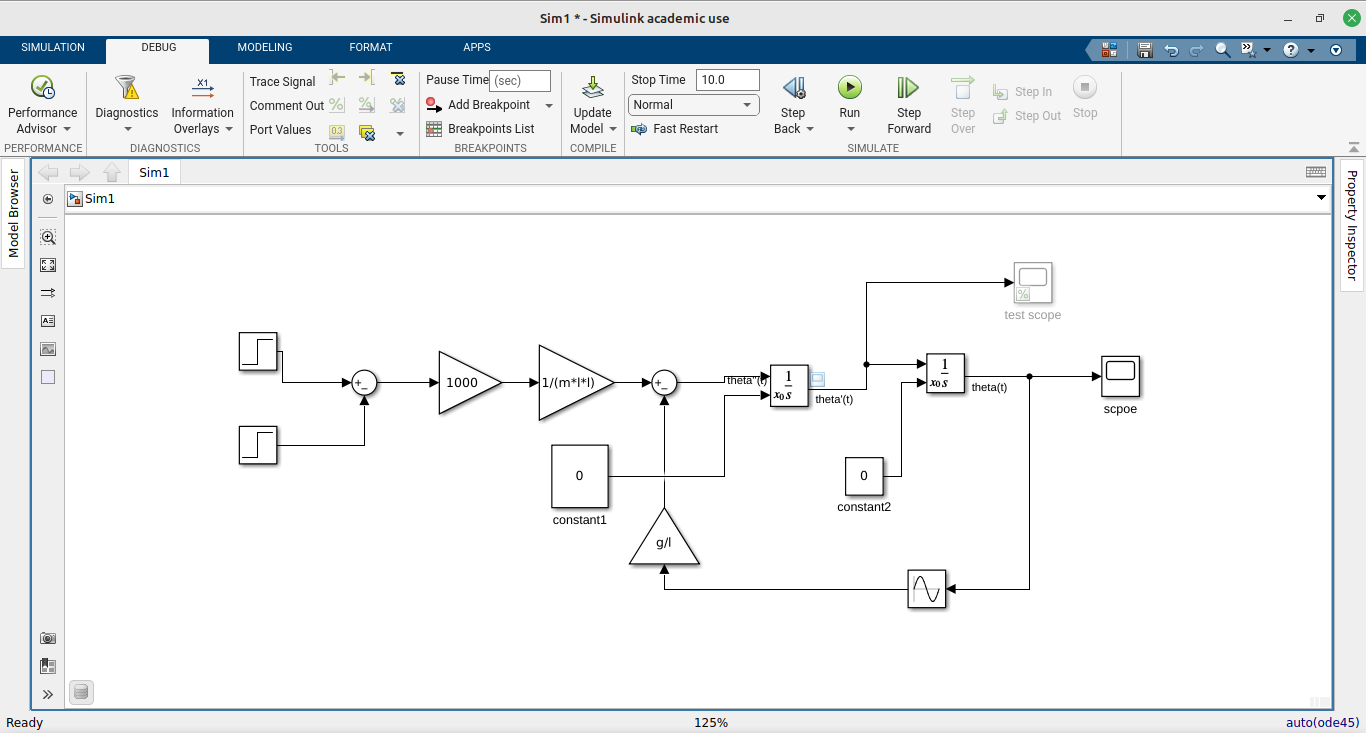
\includegraphics[width=\textwidth]{assets/hw1_sim1.png}
    \caption{diagram of simulation 1. $g=9.8$,$l=0.8$,$m=2$}
    \label{sim:1}
\end{figure}
\begin{figure}
    \centering
    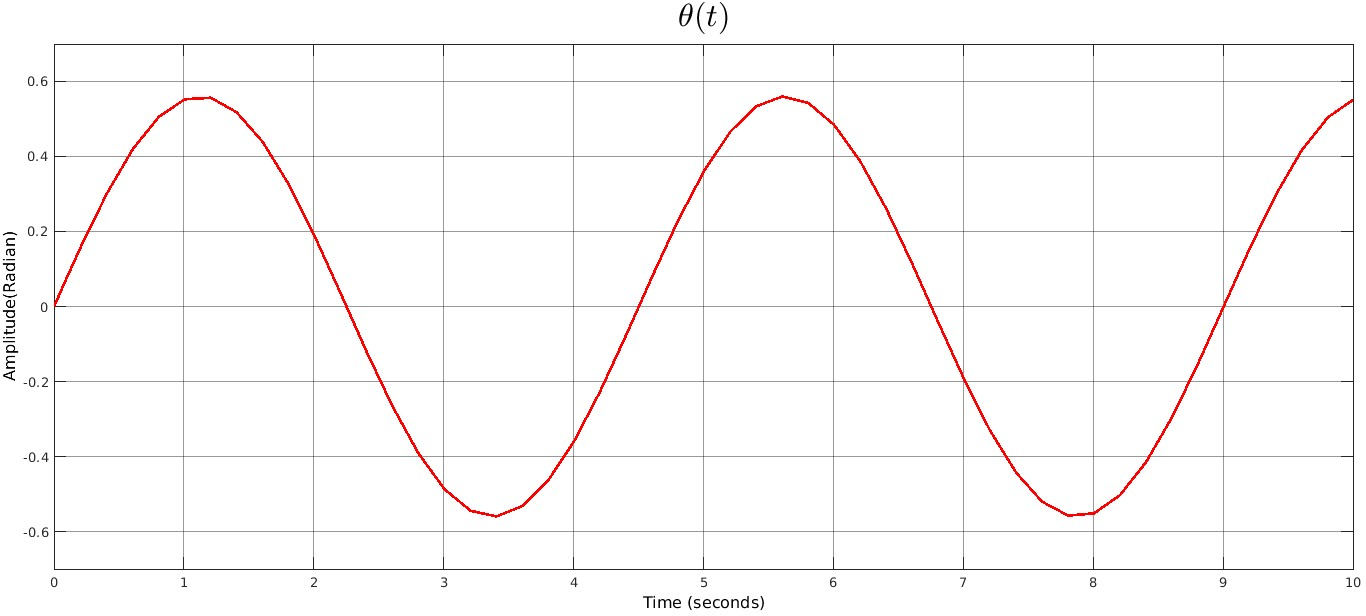
\includegraphics[width=\textwidth]{assets/hw1_3_4.jpg}
    \caption{plot of $\theta(t)$. y axes is the angle in radians and x axes is the time in seconds}
    \label{fig:sim1}
\end{figure}
\subsection{5}
Physically we can submerge the system in a viscous liquid or hang a magnetic ball near a near perfect conductor to induce eddy currents, mathematically we can add the term $-b*m*l^2\theta'(t)$ to the torque which will give us the term $-b\theta'(t)$ in the final equation.
\subsection{6}
If we want the time constant to be $10[sec]$ then from the harmonic oscillator solution we learn that we should define $b$ as $\frac{2}{10}$.

Simulation's diagram is in figure:\ref{sim:2} and graph of $\theta(t)$ is in figure:\ref{fig:sim2}. Note that $\theta(1)\approx 0.5$ and $\theta(5.6)\approx 0.3$ and if the solution has a time constant delay of $10$ seconds then $\theta(5.6)=\theta(1)\exp(-0.1(4.6))=0.31$.
\begin{figure}
    \centering
    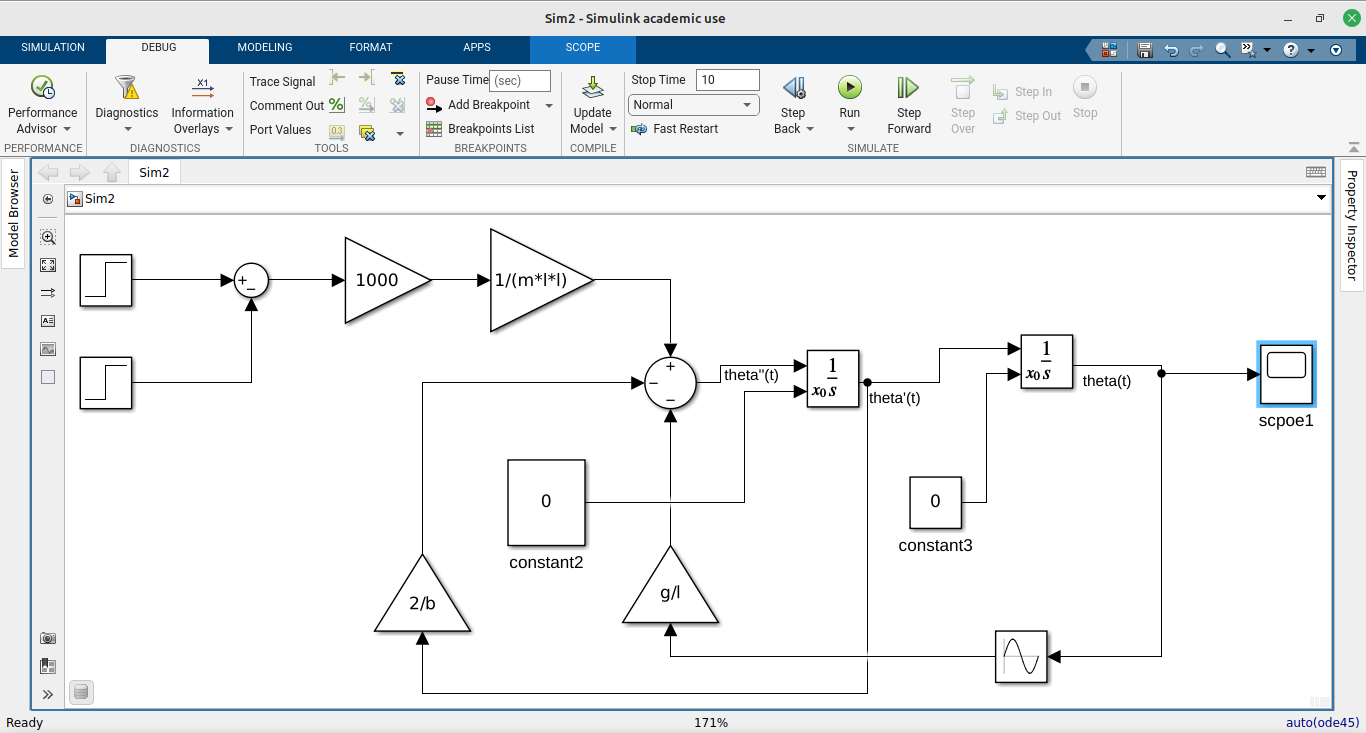
\includegraphics[width=\textwidth]{assets/hw1_sim2.png}
    \caption{diagram of simulation 2. $b=10$,$g=9.8$,$l=0.8$,$m=2$}
    \label{sim:2}
\end{figure}
\begin{figure}
    \centering
    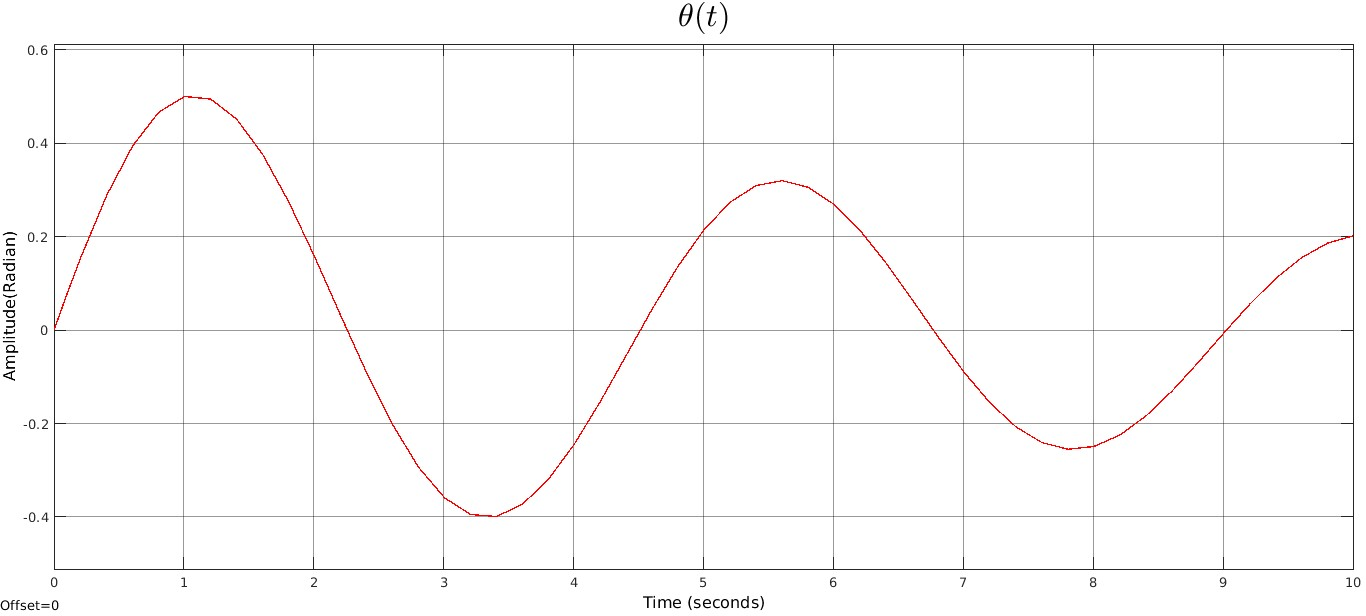
\includegraphics[width=\textwidth]{assets/hw1_3_6.jpg}
    \caption{plot of $\theta(t)$ for a damped pendulum. y axes is the angle in radians and x axes is the time in seconds}
    \label{fig:sim2}
\end{figure}